\documentclass[a4paper, 14pt]{article}
\usepackage[T2A]{fontenc}
\usepackage[utf8]{inputenc}
\usepackage[english,russian]{babel}
\usepackage[top = 2cm, bottom = 2 cm]{geometry}
\usepackage{cmap}
\usepackage{graphicx}
\usepackage{listings}
\usepackage{color}
\usepackage{amsmath}
\usepackage{pgfplots}
\usepackage{url}
\usepackage{tikz}
\usepackage{float}
\usepackage{multirow}
\usepackage{indentfirst}

\usepackage{titlesec}
\titleformat*{\section}{\LARGE\bfseries}
\titleformat*{\subsection}{\Large\bfseries}
\titleformat*{\subsubsection}{\large\bfseries}
\titleformat*{\paragraph}{\large\bfseries}
\titleformat*{\subparagraph}{\large\bfseries}


\begin{document}

	\textbf{Цель работы:} Необходимо смоделировать систему, состоящую из генератора, памяти и обслуживающего аппарата. 
	Генератор выдает сообщения, распределенные по равномерному закону, они приходят в память, обслуживающий аппарат обрабатывает каждое из них по распределению Эрланга. Необходимо определить оптимальную длину очереди, при которой не будет потеряных сообщений. Использовать принципы $\Delta t$ и событийный. Задаваемая часть сообщений попадает в очередь повторно.
	
	
	\section*{Теоретическая часть}
	\subsection*{Принцип $\Delta t$}
	
Данный принцип заключается в последовательном анализе состояний всех блоков в момент $t + \Delta t$ по заданному состоянию блоков в момент $t$. При этом новое состояние блоков определяется в соответствии с их алгоритмическим описанием с учетом действующих случайных факторов, задаваемых распределениями вероятности. В результате такого анализа принимается решение о том, какие общесистемные события должны имитироваться программной моделью на данный момент времени.

Основной недостаток этого принципа: значительные затраты машинного времени на реализацию моделирования системы. А при недостаточно малом $\Delta t$ появляется опасность пропуска отдельных событий в системе, что исключает возможность получения адекватных результатов при моделировании.

Достоинство: равномерная протяжка времени.

\subsection*{Событийный принцип}

Характерное свойство систем обработки информации заключается в том, что состояния отдельных устройств изменяются в дискретные моменты времени, совпадающие с моментами времени поступления сообщений в систему, времени поступления окончания задачи, времени поступления аварийных сигналов и т.д. Поэтому моделирование и продвижение времени в системе удобно проводить, используя событийный принцип, при котором состояние всех блоков имитационной модели анализируется лишь в момент появления какого-либо события. Момент поступления следующего события определяется минимальным значением из списка будущих событий, представляющего собой совокупность моментов ближайшего изменения состояния каждого из блоков системы.


\subsection*{Равномерное распределение}
	
Равномерное распределение - распределение случайной величины, принимающей значения, принадлежащие некоторому промежутку конечной длины, характеризующееся тем, что плотность вероятности на этом промежутке всюду постоянна.\\

Функция распределения:

\begin{equation*}
F_X (x) =
    \begin{cases}
        0, x < a \\
        \frac{x - a}{b - a}, a \le x < b \\
        1, x \geq b \\
    \end{cases}
\end{equation*}
	
Плотность распределения:

\begin{equation*}
    f_X (x) =
    \begin{cases}
        \frac{1}{b-a}, x \in [a,b] \\
        0, x \notin [a, b] \\
    \end{cases}
\end{equation*}

\newpage

\subsection*{Распределение Эрланга}

Распределение Эрланга – это гамма-распределение  с параметром $k$, принимающим лишь целые значения. \\

Функция распределения:

\begin{equation*}
F_X(x) = 1 - \sum_{i=0}^k  \frac{1}{i!} e^{-\lambda x} (\lambda x)^n
\end{equation*}
	
Плотность распределения:

\begin{equation*}
f_X(x) = \frac{\lambda^k x^{k-1} e^{-\lambda x} } {(k-1)!}
\end{equation*}


\section*{Результаты работы}

Заданные параметры:\\ \\
$a = 1,$\\
$b = 10,$\\
$k = 9,$\\
$\lambda = 0.5,$\\
$\Delta t= 0.01$\\


1000 заявок и 0\% повторов:
\begin{figure}[H]
    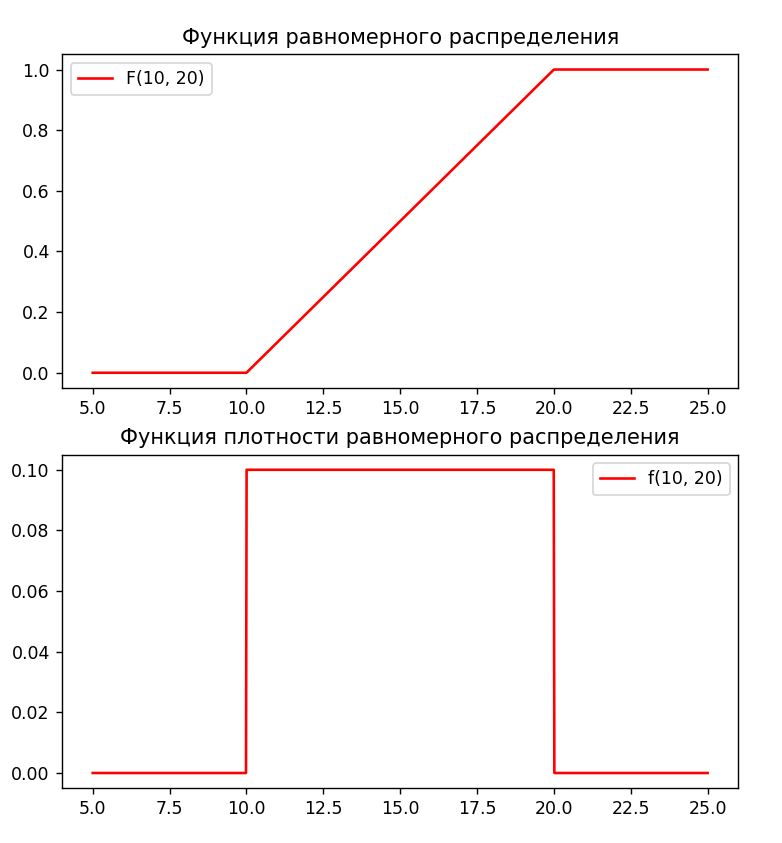
\includegraphics[scale=0.7]{1}
    \label{fig:}
\end{figure}


1000 заявок и 20\% повторов:
\begin{figure}[H]
    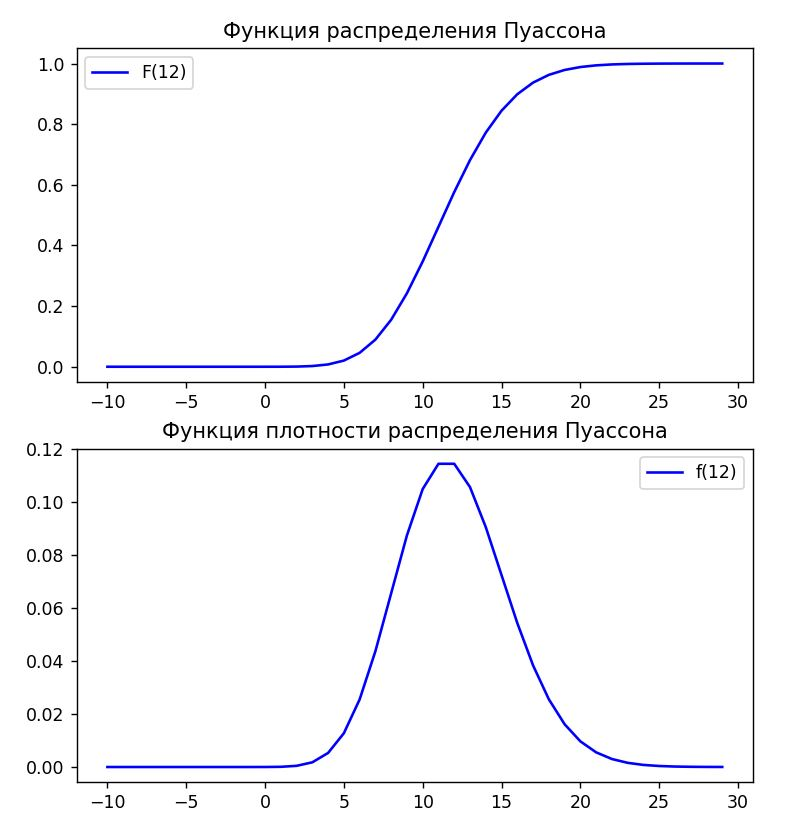
\includegraphics[scale=0.7]{2}
    \label{fig:}
\end{figure}

\newpage
1000 заявок и 50\% повторов:
\begin{figure}[H]
    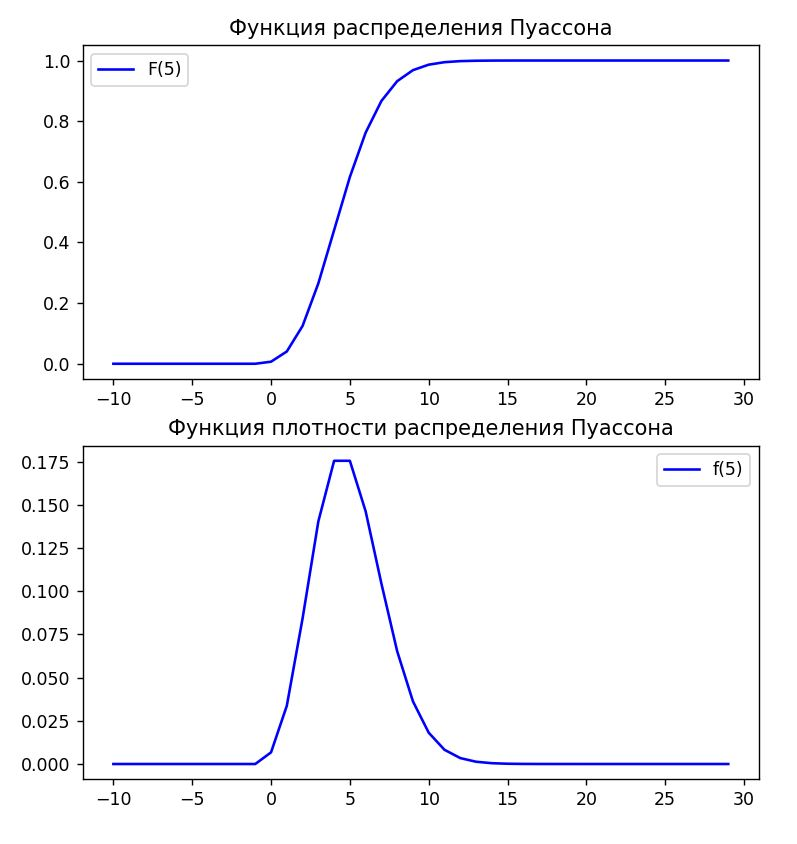
\includegraphics[scale=0.7]{3}
    \label{fig:}
\end{figure}


1000 заявок и 80\% повторов:
\begin{figure}[H]
    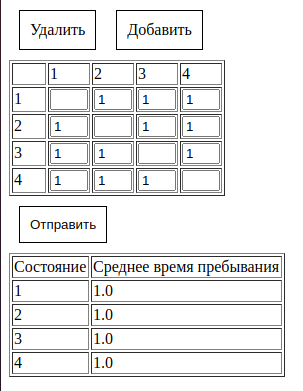
\includegraphics[scale=0.7]{4}
    \label{fig:}
\end{figure}


1000 заявок и 100\% повторов:
\begin{figure}[H]
    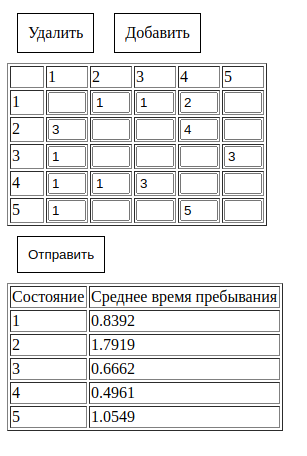
\includegraphics[scale=0.7]{5}
    \label{fig:}
\end{figure}

\newpage
10000 заявок и 0\% повторов:
\begin{figure}[H]
    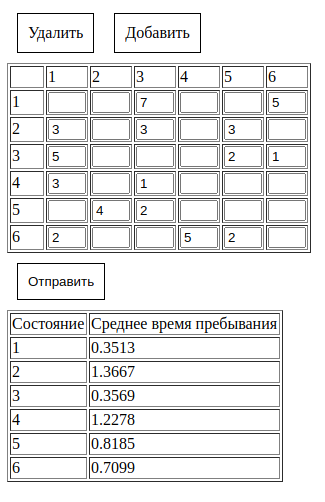
\includegraphics[scale=0.7]{6}
    \label{fig:}
\end{figure}


10000 заявок и 50\% повторов:
\begin{figure}[H]
    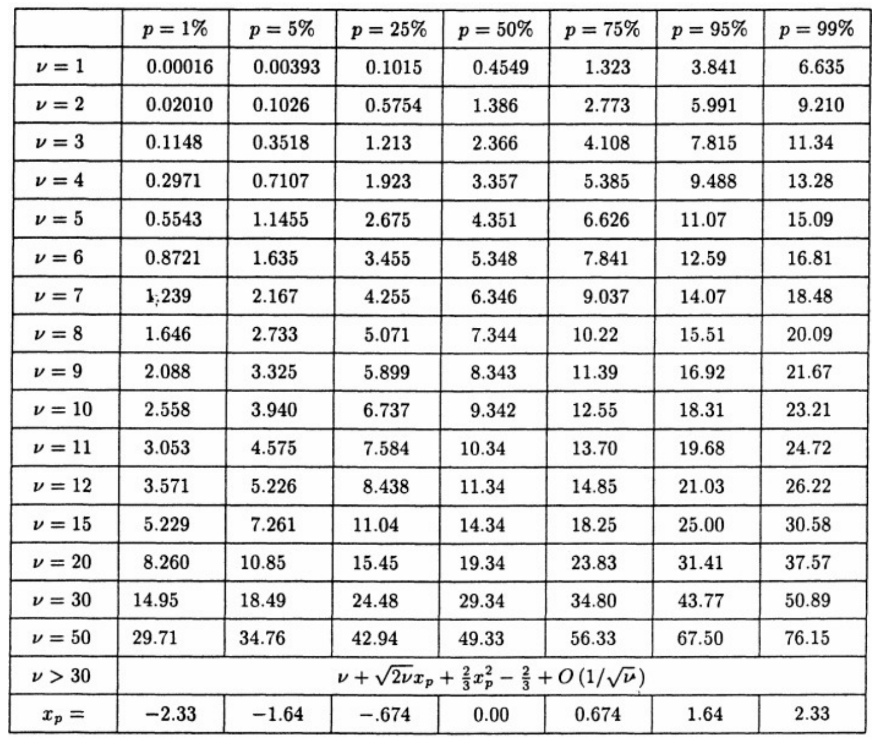
\includegraphics[scale=0.7]{7}
    \label{fig:}
\end{figure}

10000 заявок и 100\% повторов:
\begin{figure}[H]
    \includegraphics[scale=0.7]{8}
    \label{fig:}
\end{figure}


\section*{Вывод}
В ходе выполнения лабораторной работы была смоделирована система, состоящая из генератора, памяти и обслуживающего аппарата.
\end{document}